\documentclass[journal]{IEEEtran}
\usepackage[T1]{fontenc}
\usepackage{cite}
\usepackage{amsmath,amssymb,amsfonts}
\usepackage{graphicx}
\usepackage{textcomp}
\usepackage{booktabs}
\usepackage{tikz}
\usetikzlibrary{positioning,arrows.meta}
\usepackage{algorithm}
\usepackage[noend]{algpseudocode}
\algnewcommand{\Continue}{\textbf{continue}}
\usepackage{url}
\hyphenation{op-tical net-works semi-conduc-tor IEEE-Xplore Carbon-Gate}

\begin{document}

\title{Carbon-Aware GitOps Gates Revisited: A Preregistered Trace-Driven Evaluation of CarbonGate on Great Britain Grid Data}

\author{Bhavin~Kotak%
\thanks{B. Kotak is with IBM Corporation, Armonk, NY, USA (e-mail: bhavin.kotak@ibm.com; ORCID: 0009-0006-4793-7046).}%
\thanks{This is version 2.0 of the Zenodo preprint. It supersedes version 1.0, whose production evaluation figures are withdrawn.}}

\markboth{Zenodo preprint, version 2.0}{Kotak: Carbon-Aware GitOps Gates Revisited}

\maketitle

\begin{abstract}
A GitOps pipeline starts a deployment as soon as a change merges, whatever the carbon intensity of the grid at that moment. CarbonGate puts a carbon-aware admission gate in front of the GitOps reconciler. Urgent changes pass at once. Other deployments may wait for a low-intensity slot in the forecast, within a maximum-delay service-level agreement. This revision replaces the unsupported production figures of version 1 with a preregistered, trace-driven evaluation. We replay a simulated deployment workload against 12 months of half-hourly Great Britain grid data from the NESO Carbon Intensity API. The gate decides from the published forecast alone, and emissions are scored on the reported actual intensity. Over 11 held-out months and 5 seeds, forecast-based deferral with a 4 h limit cut the average-intensity emissions of deployments by 4.80\% (95\% CI 4.17 to 5.43\%), and no deployment missed its deadline. That interval contains the preregistered 5\% bound, so the primary hypothesis is inconclusive. The version 1 claim of at least 23\% is refuted. A perfect-foresight oracle reached 7.33\%. A static intensity threshold, which was the version 1 gate design, did not reduce emissions at 2 h or 4 h limits. Gains shrank as forecast error grew and were gone at a noise level of 50 gCO2/kWh. Under injected forecaster outages, fail-closed handling caused deadline violations; a cached persistence fallback still kept 4.24\% at 50\% outage. At 100 times the load, with a per-slot capacity cap, herding removed the benefit. We did not study developer acceptance.
\end{abstract}

\begin{IEEEkeywords}
Carbon-aware computing, GitOps, continuous delivery, Kubernetes, temporal workload shifting, grid carbon intensity, sustainable software engineering, trace-driven simulation.
\end{IEEEkeywords}

\IEEEpeerreviewmaketitle

\section{Introduction}
\label{sec:intro}
\IEEEPARstart{G}{itOps} treats a Git repository as the declared state of a cluster, and a controller such as Argo CD or Flux reconciles the cluster to it \cite{beetz2022gitops,argocd,fluxcd}. Continuous delivery pipelines built this way optimise for lead time and reliability \cite{shahin2017continuous}. They take no account of when the electricity for a build, test, and rollout is cleanest. Grid carbon intensity varies by hour and by season, and several systems shift flexible batch work in time to exploit that variation \cite{wiesner2021let,radovanovic2023carbon,hanafy2023carbonscaler}. Many deployments are not urgent either, so deployment pipelines are a candidate for the same idea.

Version 1 of this preprint proposed CarbonGate, a quality gate that blocks or schedules deployments according to grid intensity. Its evaluation reported production deployment counts, emission reductions, latency effects, and a developer survey. No data or code backed any of these figures, and several contradicted each other. We withdraw them here. The architectural idea stays, and the question becomes a narrower one that public data can answer. Appendix~\ref{app:changes} lists the changes.

The research question is this. If a GitOps gate defers non-urgent deployments to the lowest forecast intensity slot within a fixed maximum delay, how much does it reduce the emissions attributed to deployments, at what delay cost, and how does it behave when the forecaster fails?

We answer it with a trace-driven simulation. The grid signal is real: 12 months of half-hourly national and regional data from the NESO Carbon Intensity API \cite{nesoapi}. The deployment workload is simulated and is labelled as such. Gate decisions use only the forecast field and emissions are scored on the actual field, so the evaluation has no look-ahead leakage beyond what the published forecast itself contains. We preregistered the hypothesis, the endpoint, and the decision rule before the bulk data download.

The paper makes four contributions.
\begin{itemize}
\item A precise specification of CarbonGate as an admission policy (Section~\ref{sec:method}). It gives the system model, objective, constraints, three gate rules, and explicit behaviour for missing data, timeouts, and outages (Algorithm~\ref{alg:gate}).
\item A preregistered evaluation over 11 held-out months with 5 workload seeds that reports numerators, denominators, and 95\% confidence intervals (Section~\ref{sec:eval}).
\item Ablations that attribute the effect to forecast quality, delay budget, deferral margin, urgent share, arrival shape, and region. Stress tests cover forecaster outages and a 100-fold load increase.
\item One negative result and one inconclusive result, reported as such. The version 1 reduction claim is refuted, and the static threshold gate of version 1 did not help at short delay limits.
\end{itemize}

\section{Related Work}
\label{sec:related}
\paragraph{Temporal shifting of cloud work} Wiesner et al.\ studied how much deferrable cloud work can save by waiting for cleaner periods, using forecasts within a flexibility window \cite{wiesner2021let}. Google's carbon-intelligent computing system shapes daily datacenter capacity with day-ahead intensity forecasts \cite{radovanovic2023carbon}. CarbonScaler adapts the resource allocation of elastic batch jobs over time \cite{hanafy2023carbonscaler}, and GreenCourier applies carbon-aware placement to serverless functions \cite{chadha2023greencourier}. Sukprasert et al.\ examined the limits of temporal and spatial shifting and found that simple policies capture much of the available benefit \cite{sukprasert2024limitations}. Li et al.\ add forecast uncertainty to datacenter decarbonisation decisions \cite{li2024uncertainty}. Yang et al.\ survey carbon-aware scheduling in container orchestration \cite{yang2025survey}, and Lindberg et al.\ consider geographic load shifting \cite{lindberg2022using}. The scheduler in CarbonGate is a Let's-Wait-Awhile style deferral rule and is not new. Our contribution is to put it at the GitOps delivery gate.

\paragraph{Platform support} Bashir et al.\ argue that cloud applications should be able to see energy-system information \cite{bashir2021enabling}, and Ecovisor implements such an interface \cite{souza2023ecovisor}. Treehouse makes the general case for carbon-aware datacenter software \cite{anderson2022treehouse}. Carbon Explorer studies datacenter design under carbon objectives \cite{acun2023carbon}.

\paragraph{Carbon accounting} Kepler estimates container energy from hardware counters and models \cite{amaral2023kepler}. Green Algorithms estimates the footprint of a computation from its resource use \cite{lannelongue2021green}. Dodge et al.\ measured the operational carbon of AI workloads in cloud instances \cite{dodge2022measuring}. Embodied emissions can dominate the footprint of computing hardware, as Gupta et al.\ show \cite{gupta2021chasing}. Masanet et al.\ recalibrated global datacenter energy estimates \cite{masanet2020recalibrating}. The Software Carbon Intensity specification defines a rate-based software metric \cite{gsfsci}. Siler-Evans et al.\ distinguish marginal from average emission factors \cite{siler2012marginal}; since CarbonGate is evaluated on average intensity only, that distinction comes back in Section~\ref{sec:threats}.

\paragraph{Forecasting} CarbonCast forecasts grid carbon intensity several days ahead \cite{maji2022carboncast}. We do not build a forecaster. The gate uses the published NESO forecast, and a simple day-ahead persistence forecast is the causal comparison.

\paragraph{Delivery gates} Kubernetes dynamic admission control lets a webhook accept or reject objects at apply time \cite{k8sadmission}. GitOps controllers can delay synchronisation of a commit \cite{argocd,fluxcd}. We found no prior evaluation of carbon-aware gating at this point in the delivery path, though we do not claim that none exists.

\section{Methodology}
\label{sec:method}

\subsection{Architecture}
Fig.~\ref{fig:arch} shows where CarbonGate sits. A merged change produces a desired-state commit, and before the GitOps controller applies it, the gate classifies the deployment as urgent or deferrable. Urgent deployments pass at once. For a deferrable one, the gate queries a forecast service with a bounded timeout and returns one of three actions: deploy now, defer to a later slot, or hold and re-evaluate. The same decision function can back a pull-request status check, a delayed sync in the GitOps controller, or an admission webhook. The evaluation exercises the decision function alone, inside a replay. No live controller was involved.

\begin{figure}[!t]
\centering
\resizebox{\columnwidth}{!}{%
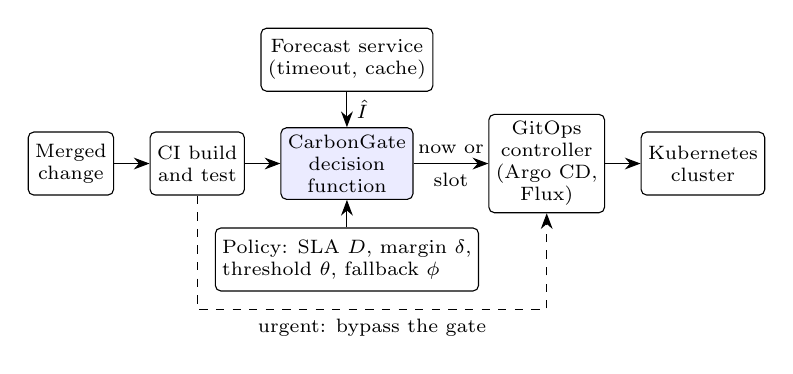
\begin{tikzpicture}[node distance=0.4cm and 0.45cm, every node/.style={font=\scriptsize},
  box/.style={draw, rounded corners=2pt, align=center, minimum height=0.8cm, inner sep=2.5pt},
  arr/.style={-{Stealth[length=2mm]}}]
\node[box] (pr) {Merged\\change};
\node[box, right=of pr] (ci) {CI build\\and test};
\node[box, right=of ci, fill=blue!8] (gate) {CarbonGate\\decision\\function};
\node[box, right=0.95cm of gate] (git) {GitOps\\controller\\(Argo CD,\\Flux)};
\node[box, right=of git] (k8s) {Kubernetes\\cluster};
\node[box, above=0.45cm of gate] (api) {Forecast service\\(timeout, cache)};
\node[box, below=0.35cm of gate, align=left] (pol) {Policy: SLA $D$, margin $\delta$,\\threshold $\theta$, fallback $\phi$};
\draw[arr] (pr) -- (ci);
\draw[arr] (ci) -- (gate);
\draw[arr] (gate) -- node[above, font=\scriptsize]{now or}node[below, font=\scriptsize]{slot} (git);
\draw[arr] (git) -- (k8s);
\draw[arr] (api) -- node[right]{$\hat I$} (gate);
\draw[arr] (pol) -- (gate);
\draw[arr, dashed] (ci.south) -- ++(0,-1.45) -| node[pos=0.25, below, font=\scriptsize]{urgent: bypass the gate} (git.south);
\end{tikzpicture}}
\caption{CarbonGate in a GitOps delivery path. Urgent deployments bypass the gate. A deferrable deployment is released now or at a later 30-minute slot picked from the forecast, subject to the maximum delay $D$.}
\label{fig:arch}
\end{figure}

\subsection{System model}
Time is divided into slots of length $\Delta = 30$ minutes, indexed by $j$. Let $I(j)$ be the realised average carbon intensity of slot $j$ in gCO$_2$/kWh, and $\hat I(j)$ the published forecast for slot $j$. Deployment $i$ arrives at time $a_i$ in slot $\sigma(a_i)$, runs for $\tau_i$ minutes, has urgency flag $u_i \in \{0,1\}$, and consumes energy $e_i$. We model energy from requested cores $c_i$ with assumed coefficients:
\begin{equation}
e_i = \rho \, \frac{\tau_i}{60} \, c_i \left(P_c + m \, P_m\right) \cdot 10^{-3}\ \text{kWh},
\label{eq:energy}
\end{equation}
where $\rho$ is the power usage effectiveness, $P_c$ the power per core in watts, $P_m$ the power per GB of memory, and $m$ the memory per core in GB. Deployment $i$, started at time $s$, emits its energy times the time-averaged intensity over its run:
\begin{equation}
C_i(s) = \frac{e_i}{\tau_i} \int_{s}^{s+\tau_i} I\big(\sigma(t)\big)\, dt .
\label{eq:emissions}
\end{equation}

\subsection{Optimisation problem}
The gate chooses a start time $s_i$ for each deployment to minimise total emissions,
\begin{equation}
\min_{\{s_i\}} \; \sum_i C_i(s_i),
\label{eq:objective}
\end{equation}
subject to the maximum-delay service-level agreement (SLA) $D$, the urgency bypass, and slot-aligned release:
\begin{equation}
\begin{aligned}
& a_i \le s_i \le a_i + D \quad \text{if } u_i = 0, \qquad s_i = a_i \quad \text{if } u_i = 1,\\
& s_i \in \{a_i\} \cup \{\, j\Delta : j > \sigma(a_i) \,\}.
\end{aligned}
\label{eq:constraints}
\end{equation}
With $K = D/\Delta$ slots of look-ahead, the candidate offsets for deployment $i$ are $k \in \{0, \dots, K\}$, where $k=0$ means starting at $a_i$. The gate has to decide online, from what is known at $a_i$, and it never sees $I(j)$ for future slots. So the rules below solve problem \eqref{eq:objective} under \eqref{eq:constraints} only approximately. The oracle solves it exactly with respect to the start-slot intensity.

\subsection{Gate rules}
Let $\hat w_i(k) = \hat I(\sigma(a_i)+k)$ be the forecast window, with missing slots excluded. CarbonGate-F (forecast deferral) picks the earliest minimiser and defers only if it beats the current slot by a margin $\delta$:
\begin{equation}
\begin{aligned}
k_i^\ast &= \operatorname*{arg\,min}_{0 \le k \le K} \hat w_i(k),\\
s_i &= \begin{cases} \big(\sigma(a_i)+k_i^\ast\big)\Delta & \text{if } k_i^\ast > 0 \text{ and}\\
 & \quad \hat w_i(k_i^\ast) \le (1-\delta)\,\hat w_i(0),\\
 a_i & \text{otherwise.}\end{cases}
\end{aligned}
\label{eq:deferral}
\end{equation}
The static threshold gate was the version 1 design. It re-checks the current-slot forecast every slot and releases at the first slot below a fixed threshold $\theta$, or at the deadline:
\begin{equation}
k_i^{\theta} = \min\Big(\{\, k \le K : \hat w_i(k) \le \theta \,\} \cup \{K\}\Big).
\label{eq:threshold}
\end{equation}
The oracle applies \eqref{eq:deferral} with $\delta = 0$ to the realised series $I$ in place of $\hat I$. It is an upper bound for start-slot deferral and cannot be deployed. The baseline, Immediate, sets $s_i = a_i$ for every deployment, which is what standard GitOps does.

\subsection{Outcome handling for the forecaster}
The forecast service is an external dependency, so the gate needs defined behaviour for when it fails. A query has one of three outcomes: \textsc{ok} with a window; \textsc{missing} when the current-slot value is null (an unknown result); or \textsc{timeout} when no answer arrives within the client budget or the service is down. A null in a future slot only removes that slot from the argmin in \eqref{eq:deferral}. On \textsc{missing} or \textsc{timeout}, the gate applies one of three fallback modes $\phi$:
\begin{equation}
\text{action} = \begin{cases}
\text{deploy now} & \phi = \text{open},\\
\text{hold, re-query next slot} & \phi = \text{closed},\\
\text{\eqref{eq:deferral} on } \hat I^{P} & \phi = \text{cached, valid},\\
\text{deploy now} & \phi = \text{cached, empty}.
\end{cases}
\label{eq:fallback}
\end{equation}
Here open, closed, and cached stand for fail-open, fail-closed, and cached persistence. Fail-closed never releases a deployment without a successful check, so it can break the SLA. The cached mode uses a day-ahead persistence forecast built from actual values fetched before the outage:
\begin{equation}
\hat I^{P}(j) = I(j - 48),
\label{eq:persistence}
\end{equation}
which is valid only if slot $j - 48$ precedes the last successful fetch.
Every SLA we test has $K < 48$, so \eqref{eq:persistence} is causal. Urgent deployments bypass the forecaster, and no forecaster outcome can delay them. Algorithm~\ref{alg:gate} puts the rules \eqref{eq:deferral}, \eqref{eq:threshold}, and \eqref{eq:fallback} together.

\begin{algorithm}[!t]
\caption{CarbonGate decision for one deployment}
\label{alg:gate}
\begin{algorithmic}[1]
\Require deployment $(a_i, u_i)$, policy $\pi$, SLA slots $K$, margin $\delta$, threshold $\theta$, fallback $\phi$
\If{$u_i = 1$ or $\pi = $ Immediate} \Return deploy now \EndIf
\State $j \gets \sigma(a_i)$; $r \gets K$
\Loop
  \State \parbox[t]{\dimexpr\linewidth-\algorithmicindent}{query forecast for slots $j..j+\max(r,0)$ with timeout budget\strut}
  \If{outcome $\neq$ \textsc{ok}}
    \If{$\phi =$ fail-open} \Return deploy now \EndIf
    \If{$\phi =$ fail-closed} \State $j \gets j+1$; $r \gets r-1$; \Continue \EndIf
    \If{cache empty} \Return deploy now \EndIf
    \State use $\hat I^{P}$ from \eqref{eq:persistence} as the window
  \EndIf
  \If{$\pi =$ CarbonGate-F} \Return offset from \eqref{eq:deferral} \EndIf
  \If{$\hat w(0) \le \theta$ or $r \le 0$} \Return deploy now \EndIf
  \State $j \gets j+1$; $r \gets r-1$ \Comment{threshold: hold}
\EndLoop
\end{algorithmic}
\end{algorithm}

\subsection{Policy as configuration}
Version 1 proposed writing the gate as a declarative policy stored next to the manifests it governs, and we keep that design. A policy object names the SLA $D$, the margin $\delta$, the optional threshold $\theta$, the fallback mode $\phi$, the forecast region, and the label that marks a deployment urgent. This object encodes the primary configuration evaluated in Section~\ref{sec:eval}:

{\footnotesize
\begin{verbatim}
kind: CarbonPolicy
spec:
  rule: forecast-deferral   # or: threshold
  maxDelay: 4h              # D
  margin: 0.05              # delta
  fallback: cached          # open | closed | cached
  forecastTimeout: 2s
  region: GB
  urgentLabel: carbongate/urgent=true
\end{verbatim}
}
The decision function in Algorithm~\ref{alg:gate} does not depend on where it runs, and there are three places it could run. A pull-request status check reports the chosen slot to the author before merge. A GitOps controller extension holds the sync of an approved commit until the slot begins. A Kubernetes validating admission webhook \cite{k8sadmission} rejects an apply that arrives before its slot. The status check is advisory only. The controller extension enforces timing without blocking authors, while the webhook enforces at the cluster boundary and also intercepts manual changes. We evaluate only the decision function; the integration points are design options, and their operational cost is untested.

\subsection{Primary metric}
For a set of deployments in a month, the relative emission reduction of a policy with start times $s_i$ is
\begin{equation}
\begin{aligned}
R &= 1 - \frac{\sum_i C_i(s_i)}{\sum_i C_i(a_i)},\\
R\big(\{\lambda e_i\}\big) &= R\big(\{e_i\}\big) \quad \text{for all } \lambda > 0.
\end{aligned}
\label{eq:reduction}
\end{equation}
The numerator is the policy's total emissions under \eqref{eq:emissions}; the denominator is the Immediate total for the same deployments. The second line holds because $C_i$ is linear in $e_i$, so a common scale factor $\lambda$ on per-deployment energy cancels. Energy is drawn independently of start time, which means $R$ does not depend on the absolute power coefficients in \eqref{eq:energy}. Absolute kilograms do depend on them. We report those separately and mark them as assumption-dependent.

\section{Evaluation}
\label{sec:eval}

\subsection{Setup}
\paragraph{Grid data} We downloaded the national intensity record (forecast and actual fields) and the regional record (forecast field only) from the NESO API \cite{nesoapi} for November 2025 to October 2026, plus one margin day. Each request covered 13 days, under the 14-day API limit. The data are licensed CC BY 4.0, and the replication package caches the raw responses with SHA-256 digests. The national record has 17568 slots. In one slot the national actual was zero; we treat a zero national actual as missing and interpolate it for scoring. Each regional series has 192 missing slots. These are interpolated for scoring and cause fail-open decisions.

\paragraph{Splits} November 2025 is the calibration month. It fixes the static threshold $\theta = 115.5$ gCO$_2$/kWh (the median forecast) and the capacity cap used in the scale test. The 11 months from December 2025 to October 2026 are held out, 16080 slots in all. No parameter was tuned on them.

\paragraph{Forecast quality} On held-out slots the NESO forecast field had a mean absolute error of 10.0 and a root mean square error of 14.4 gCO$_2$/kWh against the actual field. Day-ahead persistence had a mean absolute error of 39.9. Held-out actual intensity averaged 121.4 (standard deviation 52.5, range 20 to 286), and the mean within-day range was 99.9. For past slots the forecast field holds the last forecast issued, so its error is probably smaller than that of a forecast made hours ahead. We therefore treat it as optimistic, and bracket it with persistence and with added Gaussian noise of standard deviation $\sigma \in \{10, 25, 50\}$ gCO$_2$/kWh.

\paragraph{Simulated workload} Deployments arrive as a non-homogeneous Poisson process, at 4 per hour on weekdays from 09:00 to 18:00 Europe/London time and 0.25 per hour otherwise. Each deployment is urgent with probability $p_u = 0.10$. Durations are log-normal with a median of 15 minutes and log-standard deviation 0.5, clipped to 3 to 60 minutes. Cores are drawn from $\{0.5, 1, 2, 4\}$ with probabilities $\{0.2, 0.4, 0.3, 0.1\}$. Energy follows \eqref{eq:energy} with the version 1 coefficients $P_c = 10$ W, $P_m = 0.375$ W/GB, $m = 2$ GB, and $\rho = 1.4$. These coefficients are assumed; we did not measure them. Table~\ref{tab:config} lists the configuration. The held-out months and 5 seeds produced 50650 deployments, and 5114 of them (10.1\%) were urgent bypasses.

\begin{table}[!t]
\caption{Evaluation configuration. All values are constants in the released code.}
\label{tab:config}
\centering
\footnotesize
\begin{tabular}{@{}ll@{}}
\toprule
Item & Value \\
\midrule
Grid record & NESO national and regional, Nov 2025 to Oct 2026 \\
Slot length $\Delta$ & 30 min \\
Held-out windows & 11 calendar months; calibration Nov 2025 \\
Seeds & 0 to 4 (workload, noise, outages) \\
SLA $D$ & 2, 4 (primary), 8 h \\
Deferral margin $\delta$ & 0.05 (primary); 0, 0.10, 0.20 ablated \\
Static threshold $\theta$ & 115.5 gCO$_2$/kWh \\
Urgent share $p_u$ & 0.10 (primary); 0, 0.30 ablated \\
Outage episodes & mean 2 h; 5\%, 20\%, 50\% of slots \\
Query timeouts & independent, probability 10\% \\
Timeout budget & 2 s per forecast query \\
\bottomrule
\end{tabular}
\end{table}

\paragraph{Preregistration} Before the bulk download we fixed H1: CarbonGate-F with a 4 h SLA and the NESO forecast reduces emissions by at least 5\% relative to Immediate, with zero SLA violations. The endpoint is $R$ from \eqref{eq:reduction}, computed per held-out month and averaged over seeds, and the month is the unit of replication. We summarise it with the mean and a two-sided 95\% $t$ interval over the $n = 11$ months:
\begin{equation}
\bar R \pm t_{0.975,\,n-1}\, \frac{s_R}{\sqrt{n}} .
\label{eq:ci}
\end{equation}
H1 is supported if the lower bound of \eqref{eq:ci} exceeds 5\% and no deployment misses its deadline. It is refuted if the upper bound is below 5\% or any violation occurs, and inconclusive otherwise. H2 applies the same interval to the version 1 claim of at least 23\%. Paired comparisons between policies use per-month differences and the exact two-sided Wilcoxon signed-rank test.

\paragraph{Metrics} Besides $R$, we report the added delay $s_i - a_i$ of non-urgent deployments (median p50 and 95th percentile p95, averaged over months) and the share of non-urgent deployments deferred. We also report the share of deferrals whose emissions exceeded those of an immediate start (harmful deferrals), the SLA violation rate (violations over all deployments), the fallback rate (decisions that used a fallback, over non-urgent deployments), and absolute kilograms per seed over the 11 months.

\subsection{Results}

\paragraph{Primary endpoint} Table~\ref{tab:main} and Fig.~\ref{fig:deadline} give the main grid. With a 4 h SLA, CarbonGate-F reduced emissions by 4.80\% on average (standard deviation 0.94 across months, 95\% CI 4.17 to 5.43\%), and no deployment missed its deadline. The interval contains the preregistered 5\% bound, so H1 is \emph{inconclusive}. H2 is \emph{refuted}: the upper bound is far below 23\%. Pooled over months and seeds, the numerator was 0.369 kg and the denominator 7.52 kg of CO$_2$ per seed, for 11 months of simulated deployments. The reduction was positive in every held-out month, from 3.48\% to 6.48\% (Fig.~\ref{fig:months}).

\begin{table*}[!t]
\caption{Main results on 11 held-out months, 5 seeds each. $R$ is the relative emission reduction versus Immediate from \eqref{eq:reduction}. Delays are for non-urgent deployments. No configuration in this table violated its SLA.}
\label{tab:main}
\centering
\footnotesize
\begin{tabular}{@{}rlrrcrrrr@{}}
\toprule
$D$ (h) & Policy & $R$ mean (\%) & Std (\%) & 95\% CI (\%) & p50 delay (min) & p95 delay (min) & Deferred (\%) & Harmful (\%) \\
\midrule
2 & Static threshold & $-$0.77 & 0.97 & [$-$1.42, $-$0.12] & 27.1 & 115.3 & 46.0 & 50.4 \\
2 & CarbonGate-F & 2.41 & 0.64 & [1.98, 2.84] & 2.4 & 113.3 & 43.0 & 24.3 \\
2 & Oracle & 4.01 & 0.81 & [3.46, 4.55] & 11.5 & 114.0 & 53.4 & 0.4 \\
\midrule
4 & Static threshold & $-$0.72 & 2.49 & [$-$2.39, 0.95] & 59.4 & 234.4 & 46.0 & 48.5 \\
4 & CarbonGate-F & 4.80 & 0.94 & [4.17, 5.43] & 22.1 & 229.7 & 52.0 & 24.3 \\
4 & Oracle & 7.33 & 1.16 & [6.55, 8.11] & 38.3 & 230.4 & 59.0 & 0.3 \\
\midrule
8 & Static threshold & 2.84 & 6.33 & [$-$1.42, 7.09] & 115.8 & 473.0 & 46.0 & 38.9 \\
8 & CarbonGate-F & 10.19 & 5.37 & [6.58, 13.80] & 152.7 & 462.6 & 65.0 & 22.0 \\
8 & Oracle & 14.80 & 4.45 & [11.81, 17.79] & 166.4 & 468.8 & 71.0 & 0.2 \\
\bottomrule
\end{tabular}
\end{table*}

\begin{figure}[!t]
\centering
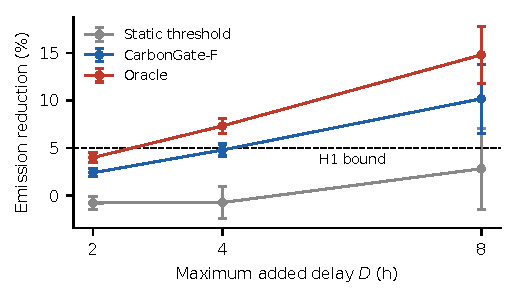
\includegraphics[width=\columnwidth]{figures/fig_deadline.pdf}
\caption{Mean held-out reduction against the maximum added delay $D$, with 95\% $t$ intervals over 11 months. The dashed line is the preregistered 5\% bound of H1.}
\label{fig:deadline}
\end{figure}

\paragraph{Delay cost} The reduction is paid for in delay. At 4 h, 52.0\% of non-urgent deployments were deferred, with a median added delay of 22.1 minutes. The 95th percentile, 229.7 minutes, was close to the 240-minute limit. CarbonGate-F captured 65.7\% of the oracle's reduction at 4 h, and the oracle beat it in every month (Wilcoxon $p = 0.001$). About a quarter of CarbonGate-F's deferrals (24.3\%) raised emissions compared with starting at once. That share reflects forecast error between slots whose intensities differ by a few gCO$_2$/kWh.

\paragraph{Longer delay budgets} With an 8 h SLA, CarbonGate-F reached 10.19\%. The month-to-month standard deviation grew to 5.37 points, though, and the p95 delay to 462.6 minutes. A longer window reaches a night or midday trough more often, but whether it gets there varies from month to month.

\paragraph{Static threshold gate} The version 1 design, rule \eqref{eq:threshold}, did not reduce emissions at 2 h or 4 h, and at 2 h its interval lies entirely below zero. It looks only at the current slot. It therefore cannot tell whether waiting will help, and 48.5\% of its deferrals were harmful at 4 h. CarbonGate-F beat it by 5.52 points at 4 h, with the paired difference in CarbonGate-F's favour in every month (Wilcoxon $p = 0.001$). In Fig.~\ref{fig:months} the threshold gate's result changes sign with the season. It was positive from December to February and negative from May to September, while its threshold stayed fixed at the November median.

\begin{figure}[!t]
\centering
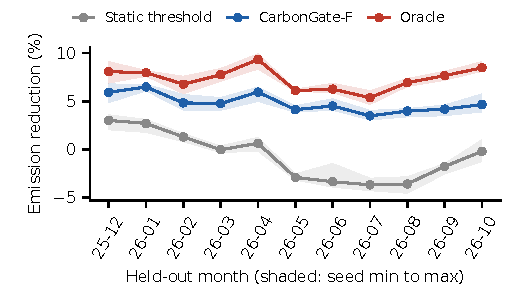
\includegraphics[width=\columnwidth]{figures/fig_months.pdf}
\caption{Reduction in each held-out month at $D = 4$ h. Lines are seed means, and the shaded bands span the 5 seeds.}
\label{fig:months}
\end{figure}

\paragraph{Where the effect comes from} Fig.~\ref{fig:profile} accounts for the size of the effect. Simulated arrivals cluster in working hours. In summer, intensity falls through the morning to a solar trough around midday and then climbs to an evening peak. A 4 h window lets morning deployments reach the trough. Afternoon deployments face rising intensity. In winter the working-hours profile is flatter. Table~\ref{tab:ablation} separates the drivers. With uniform round-the-clock arrivals CarbonGate-F reached 8.54\%, so the arrival shape alone changes the result by a large factor. Removing urgent deployments raised $R$ to 5.31\%, and a 30\% urgent share lowered it to 3.68\%. The margin $\delta$ made little difference between 0 and 0.10; at $\delta = 0.20$ both deferrals and gains fell.

\begin{figure}[!t]
\centering
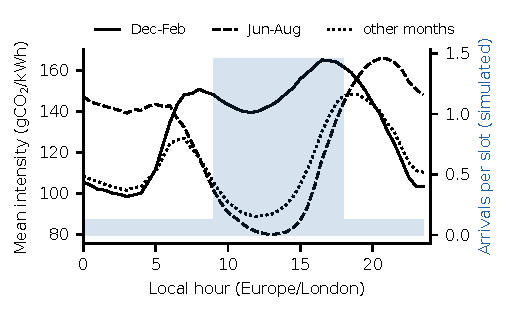
\includegraphics[width=\columnwidth]{figures/fig_profile.pdf}
\caption{Mean actual GB intensity by local hour for each season (lines, left axis) and the simulated expected arrivals per 30-minute slot (shaded, right axis).}
\label{fig:profile}
\end{figure}

\begin{table}[!t]
\caption{Ablations of CarbonGate-F at $D = 4$ h (11 held-out months, 5 seeds). $R$ is in \%, p50 delay in minutes. Deferred is a percentage of non-urgent deployments and Harmful a percentage of deferrals.}
\label{tab:ablation}
\centering
\scriptsize
\setlength{\tabcolsep}{2.2pt}
\resizebox{\columnwidth}{!}{%
\begin{tabular}{@{}llrcrrr@{}}
\toprule
Factor & Setting & $R$ & 95\% CI & p50 & Deferred & Harmful \\
\midrule
Forecast & NESO forecast (primary) & 4.80 & [4.17, 5.43] & 22.1 & 52.0 & 24.3 \\
Forecast & Day-ahead persistence & 3.65 & [3.08, 4.22] & 1.5 & 42.4 & 26.7 \\
Forecast & NESO + noise, $\sigma=10$ & 3.34 & [2.62, 4.06] & 61.8 & 68.7 & 40.4 \\
Forecast & NESO + noise, $\sigma=25$ & 1.05 & [$-$0.02, 2.12] & 78.0 & 79.5 & 48.0 \\
Forecast & NESO + noise, $\sigma=50$ & $-$1.43 & [$-$2.92, 0.06] & 88.7 & 84.5 & 53.2 \\
\midrule
Margin & $\delta=0.00$ & 4.78 & [4.08, 5.47] & 59.1 & 66.0 & 31.8 \\
Margin & $\delta=0.10$ & 4.56 & [4.02, 5.10] & 2.1 & 39.9 & 18.9 \\
Margin & $\delta=0.20$ & 3.49 & [2.96, 4.02] & 0.0 & 22.4 & 12.7 \\
\midrule
Urgent & $p_u=0.00$ & 5.31 & [4.64, 5.98] & 21.6 & 51.9 & 24.3 \\
Urgent & $p_u=0.30$ & 3.68 & [3.16, 4.20] & 21.5 & 51.9 & 24.5 \\
\midrule
Arrivals & Uniform 24/7 & 8.54 & [7.85, 9.23] & 89.2 & 62.0 & 19.9 \\
Arrivals & Uniform 24/7, oracle & 11.69 & [10.63, 12.76] & 113.9 & 70.7 & 0.2 \\
\bottomrule
\end{tabular}}
\end{table}

\paragraph{Sensitivity to the forecast} Forecast quality is the main lever. With day-ahead persistence in place of the NESO forecast, $R$ fell to 3.65\%, a paired loss of 1.16 points. Noise with $\sigma = 10$ lowered $R$ to 3.34\% and raised the harmful-deferral share to 40.4\%. At $\sigma = 25$ the interval included zero, and at $\sigma = 50$ the point estimate was negative. The NESO field for past slots is a short-lead forecast, so a deployed gate that decides hours ahead would probably land somewhere between the primary row and the noisy rows.

\paragraph{Regions} The regional endpoint publishes forecasts only. The regional test therefore scores on the regional forecast series as a proxy for actuals and decides on its day-ahead persistence. Table~\ref{tab:region} puts the result next to the national series under the same protocol. Reductions ranged from 1.81\% in North West England to 3.20\% in East England, all below the national 3.65\%. North Scotland is degenerate. Its series was zero in 84.4\% of held-out slots, so relative reductions are unstable there and only 9 months have a non-zero denominator. In absolute terms a deployment in North Scotland emits little whenever it runs. The oracle gaps are larger in the regions than nationally, which suggests that better regional forecasts would count for more than the choice of gate rule.

\begin{table*}[!t]
\caption{Regional heterogeneity at $D = 4$ h. Decisions use day-ahead persistence of each series. Scores use the regional forecast series as a proxy for actual intensity, except in the national row, which uses the actual field. Kilograms are per seed over 11 months.}
\label{tab:region}
\centering
\footnotesize
\begin{tabular}{@{}lrlrrrr@{}}
\toprule
Region & Mean intensity (gCO$_2$/kWh) & CarbonGate-F $R$ (\%) [95\% CI] & Oracle $R$ (\%) & Saved (kg) & Immediate (kg) & Months \\
\midrule
GB national & 121.4 & 3.65 [3.08, 4.22] & 7.33 & 0.274 & 7.52 & 11 \\
North Scotland & 6.6 & 0.57 [$-$1.49, 2.64] & 57.70 & 0.004 & 0.54 & 9 \\
North West England & 39.9 & 1.81 [0.13, 3.50] & 15.05 & 0.055 & 2.73 & 11 \\
South Wales & 256.1 & 3.02 [1.60, 4.44] & 9.93 & 0.437 & 15.31 & 11 \\
East England & 126.1 & 3.20 [1.88, 4.52] & 14.45 & 0.249 & 8.05 & 11 \\
London & 144.1 & 2.36 [1.60, 3.13] & 8.68 & 0.212 & 8.84 & 11 \\
\bottomrule
\end{tabular}
\end{table*}

\paragraph{Forecaster failures} Table~\ref{tab:fallback} and Fig.~\ref{fig:fallback} report the fallback tests. Fail-open kept every deployment within its SLA but lost reduction in proportion to outage time, down to 2.46\% at 50\% outage. Fail-closed broke the SLA whenever an outage lasted longer than the remaining window. At 50\% outage under CarbonGate-F, 4.55\% of all deployments missed their deadline and the longest delay was 831 minutes. The cached-persistence fallback kept 4.24\% at 50\% outage with no violations. With independent 10\% query timeouts, all three modes stayed within 4.32\% to 4.69\%; a retry one slot later usually succeeded. For the threshold gate, fail-closed caused violations in every scenario, up to 21.62\% of deployments at 50\% outage. We also probed the live forward-forecast endpoint with 20 sequential calls on 5 November 2026 (UTC). Every call succeeded. Median latency was 0.53 s, the 95th percentile 0.60 s and the maximum 0.64 s, below the 2 s budget. One probe session cannot characterise how often outages happen, so the outage rates above are stress levels. They do not estimate real outage frequency.

\begin{table*}[!t]
\caption{Forecaster outage and timeout handling at $D = 4$ h (11 held-out months, 5 seeds). FB is the share of non-urgent decisions that used the fallback (\%). Viol.\ is the share of all deployments that missed the SLA (\%). Max is the longest added delay (min).}
\label{tab:fallback}
\centering
\footnotesize
\begin{tabular}{@{}llrrrrrrr@{}}
\toprule
 & & & \multicolumn{3}{c}{CarbonGate-F} & \multicolumn{3}{c}{Static threshold} \\
\cmidrule(lr){4-6}\cmidrule(l){7-9}
Scenario & Fallback & FB (\%) & $R$ (\%) & Viol. (\%) & Max (min) & $R$ (\%) & Viol. (\%) & Max (min) \\
\midrule
Outage 5\% & Fail-open & 4.7 & 4.58 & 0.00 & 240 & $-$0.67 & 0.00 & 240 \\
 & Fail-closed & 4.7 & 4.37 & 0.47 & 848 & $-$1.02 & 1.93 & 848 \\
 & Cached & 4.7 & 4.77 & 0.00 & 240 & $-$0.66 & 0.00 & 240 \\
\midrule
Outage 20\% & Fail-open & 20.1 & 3.84 & 0.00 & 240 & $-$0.30 & 0.00 & 240 \\
 & Fail-closed & 20.1 & 3.35 & 2.04 & 970 & $-$1.40 & 8.56 & 1238 \\
 & Cached & 20.1 & 4.62 & 0.00 & 240 & $-$0.35 & 0.00 & 240 \\
\midrule
Outage 50\% & Fail-open & 49.8 & 2.46 & 0.00 & 240 & $-$0.27 & 0.00 & 240 \\
 & Fail-closed & 49.8 & 0.80 & 4.55 & 831 & $-$3.00 & 21.62 & 1078 \\
 & Cached & 49.8 & 4.24 & 0.00 & 240 & $-$0.44 & 0.00 & 240 \\
\midrule
Timeout 10\% & Fail-open & 10.2 & 4.32 & 0.00 & 240 & $-$0.58 & 0.00 & 240 \\
 & Fail-closed & 10.1 & 4.64 & 0.00 & 240 & $-$0.80 & 3.35 & 343 \\
 & Cached & 10.2 & 4.69 & 0.00 & 240 & $-$0.39 & 0.00 & 240 \\
\bottomrule
\end{tabular}
\end{table*}

\begin{figure}[!t]
\centering
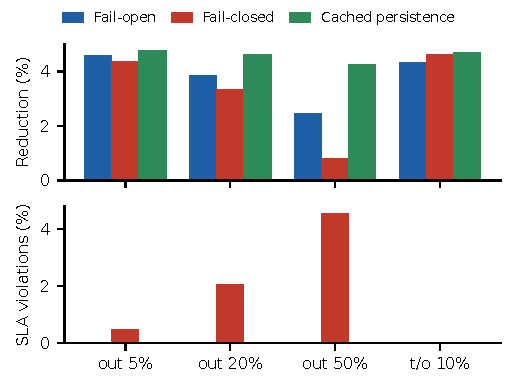
\includegraphics[width=\columnwidth]{figures/fig_fallback.pdf}
\caption{CarbonGate-F at $D = 4$ h under injected outages (out) and query timeouts (t/o). Top: mean reduction. Bottom: SLA violations as a share of all deployments.}
\label{fig:fallback}
\end{figure}

\paragraph{Herding under load} If capacity is unlimited, load does not change the relative reduction: at 100 times the arrival rate, uncapped CarbonGate-F gave 4.79\%. Capacity is the real constraint. In Table~\ref{tab:capacity}, deployment starts per slot are capped at the calibration-month peak under Immediate, which averages 7.2 at base load and 245.8 at 100 times. Uncapped deferral piled starts into the same slots, and the busiest slot reached 3.02 times the cap at base load and 6.70 times at 100 times. With the cap enforced, CarbonGate-F kept 4.62\% at base load. At 100 times the load the capped result was $-$0.95\%, with an interval spanning zero, and the median delay rose to 81.9 minutes. Early arrivals take the low-intensity slots and later ones get pushed into worse slots. A deployed gate would need capacity-aware placement or randomised release to avoid this.

\begin{table}[!t]
\caption{Load scaling with a per-slot start cap at $D = 4$ h. Peak is the number of starts in the busiest slot over the cap. $R$ is in \% with 95\% CI, and delays are in minutes.}
\label{tab:capacity}
\centering
\resizebox{\columnwidth}{!}{%
\begin{tabular}{@{}lllrlrr@{}}
\toprule
Load & Policy & Cap & Peak & $R$ [95\% CI] & p50 & p95 \\
\midrule
$\times$1 & Immediate & yes & 0.94 & 0.00 [0.00, 0.00] & 0.0 & 0.0 \\
$\times$1 & CarbonGate-F & yes & 1.00 & 4.62 [4.00, 5.24] & 25.0 & 229.9 \\
$\times$1 & CarbonGate-F & no & 3.02 & 4.80 [4.17, 5.43] & 22.1 & 229.7 \\
$\times$100 & Immediate & yes & 0.98 & 0.00 [0.00, 0.00] & 0.0 & 0.0 \\
$\times$100 & CarbonGate-F & yes & 1.00 & $-$0.95 [$-$3.62, 1.72] & 81.9 & 231.0 \\
$\times$100 & CarbonGate-F & no & 6.70 & 4.79 [4.18, 5.41] & 20.2 & 229.9 \\
\bottomrule
\end{tabular}}
\end{table}

In absolute terms, under the assumed energy model, the simulated pipeline emitted 7.52 kg of CO$_2$ per seed over 11 months under Immediate, and CarbonGate-F saved 0.369 kg of that. These values scale linearly with the assumed coefficients in \eqref{eq:energy}. They cover the deployment transient only. A deployment gate does not shift the steady-state energy of the services it deploys, so that energy is left out.

The full replay, with all ablations and the scale test, takes about a minute on a laptop CPU from cached data.

\section{Threats to Validity}
\label{sec:threats}
\paragraph{Construct validity} The metric weights energy by \emph{average} grid intensity. A change in demand alters the output of marginal generators, and their emission factor differs from the average \cite{siler2012marginal}. No free marginal series exists for GB, so marginal reductions are untested; they may be smaller or larger. Embodied emissions \cite{gupta2021chasing} and the energy of the gate itself are excluded. The energy model uses the unsourced version 1 coefficients. The relative endpoint is invariant to their scale. It is not invariant to a correlation between energy and time of day, which we did not model.

\paragraph{Forecast vintage} For past slots, the NESO forecast field holds the last forecast issued before the slot. A live gate deciding up to 8 h ahead would see larger errors. The persistence and noise ablations bound this effect from below, but we did not have the true lead-time error curve of the NESO forecast.

\paragraph{Internal validity} The workload is simulated. Arrival rates, working hours, urgent share, durations, and core counts are all assumptions, and Table~\ref{tab:ablation} shows that arrival shape changes the result substantially. Outages are synthetic renewal processes, and timeouts are independent. Real outages may be longer, or correlated with grid events. The replay also assumes that a deferred deployment always succeeds at its slot and that its rollout fits the modelled duration.

\paragraph{External validity} All results are for one grid (GB) and one year. GB has a strong solar and wind signal with a gas margin. Grids with flatter or more extreme daily profiles will give different results. Regional results score on regional forecasts as a proxy for regional actuals, which are not published. A region or country without a forecast feed would run on a fallback mode all the time.

\paragraph{Conclusion validity} The replication unit is the month, with $n = 11$, so the intervals are wide relative to the 5\% bound. Seeds vary only the simulated workload and noise. The primary hypothesis remains inconclusive, and resolving it needs more months or other grids.

\paragraph{Not tested} We did not study developer acceptance, and no users were involved. The gate was not deployed in a live Argo CD or Flux installation, so controller overheads and failure modes are unmeasured. Google's carbon-intelligent computing system \cite{radovanovic2023carbon} could not be reproduced because its capacity curves are proprietary. We did not test marginal-signal shifting in the style of commercial marginal-emission services, for lack of GB data. Capacity-aware or randomised release, which the herding result calls for, is future work. Grid feedback from many gates shifting load at once is not modelled. Embodied carbon and spatial shifting across regions were out of scope.

\section{Conclusion}
\label{sec:conclusion}
CarbonGate decides from a grid carbon forecast when a GitOps deployment may start, within a maximum-delay SLA. On 11 held-out months of real GB grid data and a simulated workload, forecast-based deferral with a 4 h limit reduced average-intensity deployment emissions by 4.80\% (95\% CI 4.17 to 5.43\%) without SLA violations. That leaves the preregistered 5\% hypothesis inconclusive and refutes the version 1 claim of at least 23\%. The static threshold gate of version 1 did not reduce emissions at 2 h or 4 h. How large the effect is depends mainly on forecast quality, the delay budget, and when deployments arrive. During outages a cached persistence fallback kept most of the reduction without SLA violations, whereas fail-closed handling traded deadline violations for little gain. Under a capacity cap at high load, naive deferral herded into the same slots and lost its benefit. Anyone adopting such a gate should prefer forecast look-ahead to fixed thresholds, use a fail-open or cached fallback, and spread releases across slots.

\paragraph*{Data and code availability} The Zenodo record for this version holds the paper source, the experiment code, the cached raw API responses with \texttt{data/SOURCES.md} (URLs, licence, retrieval dates, SHA-256 digests), all result files, the unit tests, and the preregistration. Running \texttt{python code/run\_all.py} from the package root regenerates every result, table body, and figure with fixed seeds.

\section*{Acknowledgment}
This revision was prepared with generative AI. Large language models (GitHub Copilot with Anthropic Claude) critiqued the methodology, generated the experiment code, and drafted and edited the text; in a last pass the same model also edited the wording for readability. Every reported number, table, and figure was produced by code from logged experiment results, and none was written by a language model. Grid data: Carbon Intensity API, National Energy System Operator, CC BY 4.0.

\appendices
\section{Changes from Version 1}
\label{app:changes}
\begin{itemize}
\item We withdrew the production evaluation (deployment counts, clusters, services, and period), the per-region reduction table, the latency and significance figures, the developer survey and acceptance rate, the false-positive analysis, and the cost and savings estimates. No data or code supported them, and several were mutually inconsistent.
\item We also withdrew introductory market and energy statistics that had no verifiable source, and references whose metadata matched no published record.
\item The evaluation is now a preregistered trace-driven replay on public grid data, with a labelled simulated workload, fixed seeds, held-out months, and confidence intervals.
\item The gate architecture, the policy-as-configuration idea, and the integration points are kept. The scheduler is now written as an explicit rule, \eqref{eq:deferral}, next to the version 1 threshold rule, \eqref{eq:threshold}.
\item New in this version are defined behaviour for forecaster failures, \eqref{eq:fallback}, tested under injected outages; a load-scaling test with a capacity cap; and a threats section that lists untested items.
\item The headline result changed. Version 1 reported reductions of at least 23\%. This version measures 4.80\% for the primary configuration and refutes that claim for the setting studied.
\end{itemize}

\bibliographystyle{IEEEtran}
\bibliography{references}

\end{document}
